%
% chapter.tex -- Kapitel 2: Koordinaten und Tangentialvektoren
%
% (c) 2024 Prof Dr Andreas Müller
%
\chapter{Koordinaten und Tangentialvektoren
\label{chapter:koordinaten}}
\kopflinks{Koordinaten und Tangentialvektoren}
Die Bühne der Physik ist ein Raum von Punkten, in dem wir geometrische
Konstruktionen anwenden und zum Beispiel Bahnen von Körpern beschreiben
können.
Solche Beschreibungen verwenden immer mehr oder weniger speziell gewählte
Koordinatensysteme, die Punkte durch Koordinaten beschreiben.
Da die Koordinaten nur ein Werkzeug zur physikalischer Gegebenheiten
sind, muss es immer möglich sein, die zur Formulierung von Naturgesetzen
entwickelten Abstraktionen wie Kurven, Funktionen oder Vektoren zwischen
beliebigen Koordinatensystemen umzurechnen.
Ziel dieses Kapitels ist daher, eine für alle Arten von Koordinatensystemen
nützliche Notation zu entwickeln, die Umrechnung zwischen Koordinatensystemen
zu studieren und den Begriff des Tangentialvektors einzuführen.

%
% Koordinaten
%
\section{Koordinaten
\label{buch:koordinaten:section:koordinaten}}
\kopfrechts{Koordinaten}
In diesem Abschnitt betrachten wir eine Punktmenge $X$, die mit
Koordinatensystemen ausgestattet werden soll.
Ohne das Koordinatensystem hat die Punktemenge keinerlei Struktur.
Um von stetigen Abbildungen zwischen solchen Mengen zu sprechen,
wird zum Beispiel ein Begriff der Nähe benötigt, mit dem die Konvergenz
von Folgen definiert werden kann.
Die Konstruktion eines Koordinatensystems ermöglicht, Punkte also
nahe beeinander zu betrachten, wenn sich ihre Koordinaten nur geringfügig
unterscheiden.

%
% Koordinatensystem
%
\subsection{Koordinatensystem}
%
% fig-koordinaten.tex
%
% (c) 2024 Prof Dr Andreas Müller
%
\begin{figure}
\centering
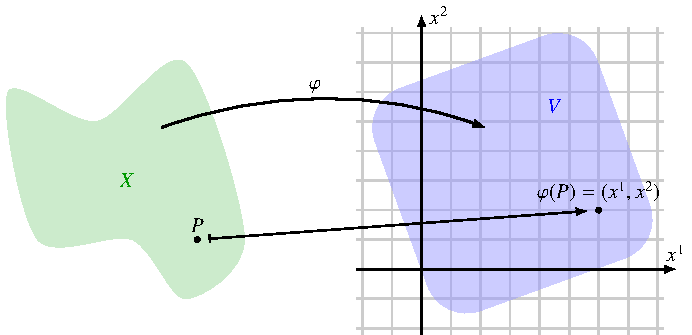
\includegraphics{chapters/020-koordinaten/images/koordinaten.pdf}
\caption{Ein Koordinatensystem auf der Punktmenge $X$ ist eine Abbildung 
$\varphi$ in den Koordinatenraum $V$, der eine Teilmenge von
$\mathbb{R}^n$ ist.
\label{buch:koordinaten:koordinaten:fig:koordinaten}}
\end{figure}
%
Ein $n$-dimensionales Koordinatensystem auf $X$ ordnet jedem Punkt 
ein $n$-Tupel von Koordinaten zu.
Aus erst später verständlichen Gründen bezeichnen wir die Koordinaten
mit hochgestellten Indizes, wir schreiben also $x^1,\dots,x^n$.
Eine Verwechslungsgefahr mit Exponenten besteht normalerweise nicht.
Falls die $k$-te Potenz der Koordinate $x^1$ berechnet werden soll, 
wird dies mit Klammern als $(x^i)^k$ geschrieben.
Ein Koordinatensystem ist also eine Abbildung
\[
\varphi
\colon
X\to \mathbb{R}^n
:
P \mapsto (x^1,\dots,x^n),
\]
wie sie in Abbildung~\ref{buch:koordinaten:koordinaten:fig:koordinaten}
dargestellt ist.
Jede einzelne Koordinate kann als Funktion $P\mapsto x^i(P)$ mit
reellen Werten betrachtet werden.

\begin{beispiel}
\label{buch:koordinaten:koordinaten:beispiel:kartpolar}
%
% fit-kartpolar.tex%
%
% (c) 2024 Prof Dr Andreas Müller
%
\begin{figure}
\centering
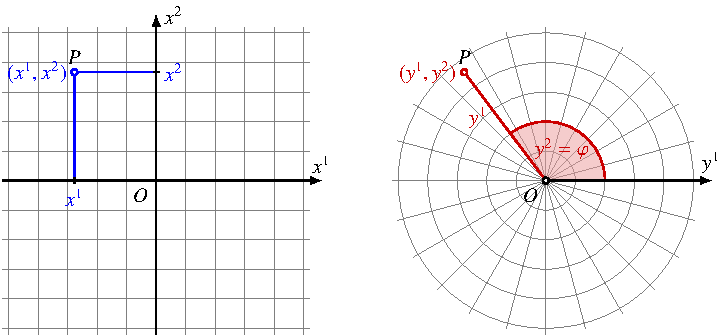
\includegraphics{chapters/020-koordinaten/images/kartpolar.pdf}
\caption{Zwei Koordinatensysteme für die Ebene:
kartesische (rechtwinklige) Koordinaten links und Polarkoordinaten
rechts.
Der gleiche Punkt $P$ wird gleichermassen durch die Koordinaten 
$(x^1,x^2)$ und $(y^1,y^2)$ beschrieben.
\label{buch:koordinaten:fig:kartpolar}}
\end{figure}

Die Punkte einer Ebene können einerseits mit dem {\em kartesischen}
Koordinatensystem mit den Koordinaten $(x^1,x^2)\in\mathbb{R}$ 
beschrieben werden und andererseits durch {\em Polarkoordinaten},
\index{Polarkoordinaten}%
die einen Punkt durch den Radius $y^1 = r$ und den Polarwinkel
$y^2 = \varphi$ definieren (Abbildung~\ref{buch:koordinaten:fig:kartpolar}).

Die kartesischen Koordinaten können aus den Polarkoordinaten durch
\begin{equation}
\left.
\begin{aligned}
x^1 &= y^1\cos y^2 \\
x^2 &= y^1\sin y^2
\end{aligned}
\qquad
\right\}
\label{buch:koordinaten:koordinaten:eqn:polarkartumrechnung}
\end{equation}
berechnet werden.
\end{beispiel}

\begin{beispiel}
\label{buch:koordinaten:koordinaten:beispiel:kartkugel}
%
% fig-kartkugel.tex
%
% (c) 2024 Prof Dr Andreas Müller
%
\begin{figure}
\centering
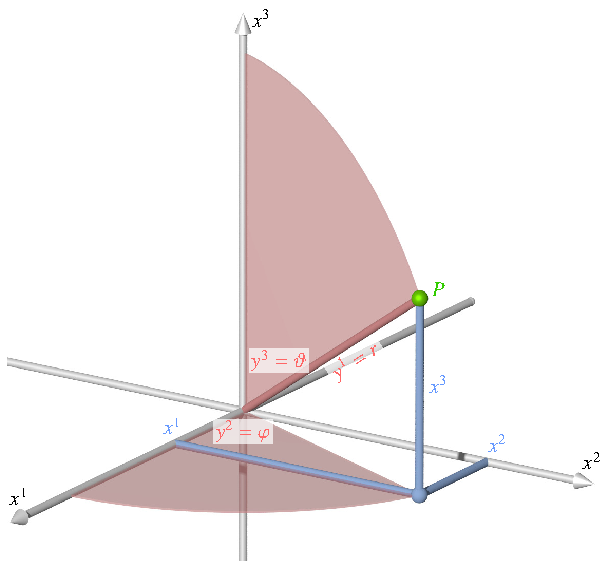
\includegraphics{chapters/020-koordinaten/images/kartkugel.pdf}
\caption{Kartesische Koordinaten ({\color{blue}blau}) und Kugelkoordinaten
({\color{darkred}rot}) für einen Punkt $P$ des dreidmensionalen Raumes.
\label{buch:koordinaten:koordinaten:fig:kartkugel}}
\end{figure}

Der dreidimensionale Raum kann sowohl durch {\em kartesische}
Koordinatentripel $(x^1,x^2,x^3)$ wie auch durch {\em Kugelkoordinaten}
\index{Kugelkoordinaten}%
beschrieben werden.
In Kugelkoordinaten ist ein Punkt durch die Entfernung $r=y^1$ vom
Nullpunkt, den Polarwinkel $y^2=\varphi$ seiner Projektion in die 
$x^1$-$x^2$-Ebene und den Winkel $\vartheta$ zwischen der positiven
$x^3$-Achse und der Geraden durch Nullpunkt $O$ und den Punkt gegeben
(Abbildung~\ref{buch:koordinaten:koordinaten:fig:kartkugel}).
Die Umrechnung von Kugelkoordinaten in kartesische Koordinaten
erfolgt mit
\begin{equation}
\left.
\begin{aligned}
x^1
&=
y^1 \cos y^2 \cos y^3 \\
x^2
&=
y^1 \sin y^2 \cos y^3 \\
x^3
&=
y^2 \cos y^3.
\end{aligned}
\qquad\right\}
\label{buch:koordinaten:koordinaten:eqn:kugelkartumrechnung}
\end{equation}
Man beachte, dass Punkte auf der $x^3$-Achse $y^3=0$ oder
$y^3=\pi$ und beliebigen Winkel $y^2\in\mathbb{R}$ haben.
Ohne zusätzliche Einschränkungen haben die Punkte auf der
$x^3$-Achse keine eindeutigen Kugelkoordinaten.
\end{beispiel}

Um die Struktur des Koordinatenraumes $\mathbb{R}^n$ auf die Menge
$X$ zu übertragen, müssen die Koordinatenabbildungen weiter eingeschränkt
werden.
Zunächst muss die Koordinatenabbildung bijektiv sein.
Dies bedeutet, dass jeder Punkt durch genau ein Koordinaten-$n$-Tupel
beschrieben wird.
Diese Bedingung ist in beiden Beispielen nicht erfüllt, da Tupel,
deren $y^2=\varphi$-Koordinaten sich um $2\pi$ unterscheiden, den
gleichen Punkt beschreiben.
Sie ist aber für genügend kleine Teilmengen des Raumes erfüllt.

Tatsächlich kann man nicht erwarten, zum Beispiel die Oberfläche einer
Kugel oder eines Torus in ihrer Gesamtheit eineindeutig auf Ebene
abzubilden.
Die Definition eines Koordinatensystems ist vorerst also nur geeignet,
eine Punktmenge lokal zu beschreiben.
Für eine globale Beschreibung wird es notwendig sein, verschiedene
Koordinatensysteme, die auf Teilen einer Menge definiert sind, zu
einem grösseren Ganzen zusammenzufügen.

Ausserdem muss die Menge $V=\varphi(X)$ der möglichen Koordinaten-$n$-Tupel
eine offene Menge in $\mathbb{R}^n$ sein.
Auch diese Bedingung ist in den Beispielen nicht erfüllt.
Die $y^1=r$-Koordinate nimmt alle Werte in
\[
\mathbb{R}_{\ge 0}
=
[0,\infty)
=
\{
y^1\in\mathbb{R}
\mid
y^1\ge 0
\}.
\]
Dies ist keine offene Menge, da die Punkte $(0,y^2)$ bzw.~$(0,y^2,y^3)$
ein Randpunkt des Wertebereichs der $y$-Koordinaten ist.
Bei Kugelkoordinaten nimmt die Koordinate $y^3$ Werte im
abgeschlossenen Interval $[0,\pi]$ an, was zu weiteren Randpunkten
des Wertebereichs führen.

% XXX Beispiel zur Notwendigkeit der letzten Bedingung zeigen

%
% Koordinatenwechsel
%
\subsection{Koordinatenwechsel}
In den Beispielen
\ref{buch:koordinaten:koordinaten:beispiel:kartpolar}
und
\ref{buch:koordinaten:koordinaten:beispiel:kartkugel}
wurden bereits Umrechnungsformeln zwischen den dort dargestellten
Koordinatensystemen ermittelt.
Seien etwas allgemeiner zwei Koordinatensysteme $x^1,\dots,x^n$
und $y^1,\dots,y^n$ auf der Punktmenge $X$ gegeben.
Sei $W$ die Menge der Koordinaten-$n$-Tupel, die Punkte von $X$
in den $x^i$-Koordinaten beschreiben, also die Bildmenge der
Koordinatenabbildung $\varphi$.
Sei weiter $\psi$ die Koordinatenabbildung für die $y^i$-Koordinaten
und $W$ der zugehörige Wertebereich.
Dann ist die Umkehrabbildung $\varphi^{-1}$ auf $U$ definiert durch die
Zusasmmensetzung
\[
\psi
\circ
\varphi^{-1}
\colon
U\to V\subset\mathbb{R}^n
:
(x^1,\dots,x^n)
\mapsto
(y^1,\dots,y^n).
\]
Dies ist die Koordinatenumrechnung vom $x^i$-Koordinatensystem in
das $y^i$-Koordinatensystem, eine Abbildung von $U$ in $V\subset\mathbb{R}^n$.

% XXX Koordinatenwechsel-Abbildung

Die Koordinatenwechsel-Abbildung ist umkehrbar, da sowohl $\varphi$
als auch $\psi$ umkehrbar sind.
Die Umkehrabbildung ist die Abbildung
\[
(\psi\circ\varphi^{-1})^{-1}
=
\varphi\circ\psi^{-1}
\colon
V\to W \subset \mathbb{R}^n.
\]
%
% Stetigkeit
%
\subsubsection{Stetigkeit}
Die Koordinatenabbildungen $\varphi$ ermöglicht, auf der Menge
$X$ zu definieren, was eine konvergente Folge ist.
Die Punkte $P_k\in X$ konvergieren genau dann gegen den Punkt $P$,
wenn die Bildpunkte $\varphi(P_k)$ in $U$ gegen $\varphi(P)$
konvergieren.

Eine weitere Koordinatenabbildung $\psi\colon X\to V$ definiert einen
weiteren Begriff der Konvergenz von Punktfolgen in $X$.
Die Eigenschaft einer Folge, zu konvergieren, sollte nicht davon 
abhängig sein, in welchen Koordinaten der Grenzwert berechnet
werden soll.
Für jedes Koordinatensystem sollte sich der gleiche Begriff der
Konvergenz von Folgen ergeben.
Dies schränkt die Menge der zulässigen Koordinatensysteme ein.

Zwei Koordinatensysteme $\varphi$ und $\psi$ führen auf den gleichen
Konvergenzbegriff, wenn für jede Folge $P_k\in X$ die Folgen
\[
x_k=\varphi(P_k)\in V
\qquad\text{und}\qquad
y_k=\psi(P_k)\in W
\]
beide konvergent oder beide nicht konvergent sind.
Dies trifft genau dann zu, wenn die Koordinatenwechselabbildungen
$\psi\circ\varphi^{-1}$ in jedem Punkt stetig sind.

Konvergenz einer Folge in $\mathbb{R}^n$ wird die Entfernung von Punkten 
\[
d(P,Q)
=
|x(P)-x(Q)|
\]
bestimmt.
Die Funktion $d$ heisst auch die vom Koordinatensystem induzierte 
{\em Metrik}.
\index{Metrik}%
Eine Folge $P_k$ konvergiert gegen $P$, wenn es für jedes $\varepsilon>0$
eine Zahl $N$ gibt derart, dass der Abstand $d(P,P_k)<\varepsilon$, wenn
$k>N$ ist.
Der Begriff des Abstandes von Punkten lässt sich mit der Koordinatenabbildung
nicht auf die Menge $X$ übertragen, da die Abstände je nach Koordinatensystem
verschieden sein können.
Dies ist aber auch nicht nötig, denn Konvergenz verlangt nur, dass genügend
kleine Abstände in einem Koordinatensystem auch genügend klein sind in jedem
anderen Koordinatensystem.
Die Koordinatenwechselabbildung $\psi\circ\varphi^{-1}$  muss daher die
Bedingung erfüllen, dass es für jedes $\varepsilon>0$ ein $\delta>0$ gibt,
dass 
\[
|y(P)-y(Q)| < \varepsilon
\]
für alle Paare von Punkten $P$ und $Q$ mit $|x(P)-x(Q)| < \delta$
gilt.
Dies ist aber die Definition einer stetigen Abbildung.

\begin{definition}[offene Menge in $X$]
\label{buch:koordinaten:koordinaten:definition:offenemenge}
Eine Menge $U\subset X$ heisst eine {\em offene Menge}, wenn es für jeden Punkt
\index{offene Menge}%
\index{Menge!offen}%
$P\in X$ und für jedes Koordinatensystem $\varphi:\colon X\to V$
ein $\varepsilon >0$ gibt derart, dass die Menge
\[
U_{P,\varphi}
=
\varphi^{-1}\bigl(
\{
x\in V
\mid
|x-\varphi(P)|<\varepsilon
\}
\bigr)
\]
in $U$ enthalten ist: $U_{P,\varphi}\subset U$.
\end{definition}

Die Definition transportiert die Idee einer kleinen Umgebung
eines Punktes mithilfe der Koordinatenabbildung von der Bildmenge
$V\subset \mathbb{R}^n$ auf die Menge $X$.
Damit sich daraus ein konsistenter Begriff der kleinen Umgebung 
ergibt, müssen verschiedene Koordinatensysteme die gleichen
kleinen Umgebungen erzeugen.
Dies wird durch die folgende Definition sichergestellt.

\begin{definition}[stetige Struktur]
\label{buch:koordinaten:koordinaten:definition:stetigestruktur}
\index{stetige Struktur}%
\index{Struktur!stetig}%
Eine {\em stetige Struktur} auf der Punktemenge $X$ ist eine mit
der Indexmenge $I$ indizierte Familie
\[
\varphi_\alpha\colon X\to V_\alpha \subset \mathbb{R}^n,
\]
$\alpha\in I$,
von Koordinatensystemen auf der Menge $X$ derart, dass die
Koordinatenwechselabbildungen
\[
\varphi_{\beta}\circ\varphi_\alpha^{-1}
\colon
V_\alpha \to V_\beta
\]
stetige Abbildungen für alle $\alpha,\beta\in I$ sind.
\end{definition}

Mit jedem Koordinatenwechsel ist auch die Umkehrabbildung ein
Koordinantenwechsel.
Die Koordinatenwechsel sind also alle umkehrbare stetige Abbildungen,
oder {\em Homöomorphismen}.

Will man ein neues Koordinatensystem auf $X$ verwenden, muss es so
gewählt werden, dass es mit allen bereits verwendeten Koordinatensystemen
verträglich ist.
Die Koordinatenwechsel von und zum neuen Koordinatensystem müssen
alle stetig sein.

%
% Stetige Funktionen auf X
%
\subsubsection{Stetige Funktionen auf $X$}
Sei jetzt $f\colon X\to\mathbb{R}$ eine reellwertige Funktion.
Ohne ein Koordinatensystem ist nicht klar, was es heissen soll, dass die
Funktion $f$ stetig ist.
Mit Hilfe eines Koordinatensystems $\varphi\colon X\to V$ kann man die
Funktion $f$ jetzt auch in Koordinaten schreiben.
Dazu bildet man die Funktion
\[
f_\varphi
=
f\circ \varphi^{-1}
\colon
V
\to
\mathbb{R}
:
(x^1,\dots,x^n)
\mapsto
f(\varphi^{-1}(x^1,\dots,x^n))
=
f(x^1,\dots,x^n).
\]
Eine Funktion $f$ heisst stetig, wenn die in $x$-Koordinaten geschriebene
Funktion $f(x^1,\dots,x^n)$ eine stetige Funktion ist.
Wählt man ein anderes Koordinatensystem $\psi\colon X\to W$ einer
stetigen Struktur auf $X$, dann ist der Koordinatenwechsel
$\varphi\circ\psi^{-1}$ in Homöomorphismus, insbesondere ist 
\[
f_\psi
=
f\circ\psi^{-1}
=
\underbrace{f\circ\varphi^{-1}}_{\displaystyle f_\varphi\mathstrut}
\circ
\underbrace{\varphi\circ\psi^{-1}}_{\displaystyle
\hbox to6pt{\rlap{\text{Koordinatenwechsel\strut}}\hfill}}
\colon
W\to \mathbb{R}
\]
genau dann stetig, wenn auch $f_\varphi$ stetig ist.
Eine stetige Struktur auf $X$ ermöglicht also insbesondere auch,
auf konsistente Weise über Stetigkeit von rellwertigen Funktionen
auf $X$ zu sprechen.

%
% Differenzierbarkeit
%
\subsubsection{Differenzierbarkeit}
Für eine beliebige Punktmente $X$ ist es im Allgemeinen nicht sinnvoll,
von differrenzierbaren Funktionen zu sprechen.
Die Existenz der Ableitung $f'(x_0)$ einer Funktion im Punkt $x_0$
basiert darauf, dass es eine lineare Ersatzfunktion
\begin{equation}
f(x) = f(x_0) + f'(x_0)\cdot (x-x_0)+o(x-x_0)
\label{buch:koordinaten:koordinaten:eqn:linersatz}
\end{equation}
gibt.
Die Darstellung~\eqref{buch:koordinaten:koordinaten:eqn:linersatz}
ist nur sinnvoll, wenn der Definitions- wie auch der Wertebereich
Teilmengen von $\mathbb{R}$ sind.

Eine Funktion $f\colon X\to \mathbb{R}$ kann in einem Koordinatensystem
$\varphi\colon X\to V\subset\mathbb{R}^n$ als Funktion
\[
f_\varphi
\colon
V\to\mathbb{R}
:
(x^1,\dots,x^n)
\mapsto
f\circ\varphi^{-1}(x^1,\dots,x^n)
\]
der Koordinaten $x^i$ geschrieben werden.
Damit ist die Voraussetzung geschaffen, von den Ableitungen von $f$
nach jeder beliebigen Koordinate zu sprechen.
Die {\em partielle Ableitung} von $f$ nach der Koordinaten $x^i$ im
Koordinatensystem $\varphi$ ist
\begin{equation}
\frac{\partial f}{\partial x^i}
=
\frac{\partial f_\varphi}{\partial x^1}(x^1,\dots,x^n)
=
\lim_{h\to 0}
\frac{f_\varphi(x^1,\dots,x^i+h,\dots, x^n)-f(x^1,\dots,x^n)}{h}.
\label{buch:koordinaten:koordinaten:eqn:partabl}
\end{equation}
Bei der Ableitung werden alle Koordinaten ausser der Koordinaten $x^i$
konstant gehalten.

Der Ausdruck~\eqref{buch:koordinaten:koordinaten:eqn:partabl} ist ganz
explizit von der Wahl des Koordinatensystems abhängig.
Sei $\psi\colon X\to W$ ein weiteres Koordinatensystem, dann lassen sich
die Koordinaten $x^i$ des Koordinatensystems $\varphi$ in die 
Koordinaten $y^k$ des Koordinatensystems $\psi$ umrechnen.
Die Koordinate $y^k$ ist eine reellwertige Funktion auf $X$, wir
können daher auch die partiellen Ableitungen
\[
\frac{\partial y^k}{\partial x^i}(x^1,\dots,x^n)
\]
bilden.
Aus der Kettenregel können jetzt die partiellen Ableitung bezüglich
der Variablen $y^k$ durch die partiellen bezüglich der Variablen $x^i$
als
\begin{align*}
\frac{\partial}{\partial x^i}
(f\circ\psi^{-1})\circ (\psi\circ\varphi^{-1})(x^1,\dots,x^n)
&=
\sum_{k=1}^n
\frac{\partial f\circ\psi^{-1}}{\partial y^k}(y^1,\dots,y^n)
\cdot
\frac{\partial y^k}{\partial x^i}(x^1,\dots,x^n)
\end{align*}
ausgedrückt werden.

\begin{definition}[Jacobi-Matrix]
Die Matrix
\[
J
=
\frac{\partial(y^1,\dots,y^n)}{\partial(x^1,\dots,x^n)}
=
\bgroup
\renewcommand\arraystretch{1.8}
\begin{pmatrix}
\displaystyle\frac{\partial y^1}{\partial x^1}&\dots&\displaystyle\frac{\partial y^1}{\partial x^n}\\
\vdots&\ddots&\vdots\\
\displaystyle\frac{\partial y^n}{\partial x^1}&\dots&\displaystyle\frac{\partial y^n}{\partial x^n}\\
\end{pmatrix}
\egroup
\]
mit den Matrixeinträgen
\[
J_{ki}
=
\frac{\partial y^k}{\partial x^i}(x^1,\dots,x^n)
\]
heisst die {\em Jacobi-Matrix} der Funktionen $y^k(x_1,\dots,x_n)$.
\index{Jacobi-Matrix}%
\end{definition}

Die Umrechnung der partiellen Ableitungen zwischen verschiedenen
Koordinatensystemen erfolgt also mit Hilfe der Jacobi-Matrix der
Koordinatentransformation.

\begin{definition}
Ein Koordinatenwechsel $\psi\circ\varphi^{-1}$ heisst
{\em stetig differenzierbar}, wenn die Jacobi-Matrix $J$
stetig ist.
\end{definition}

Die Eigenschaft der Differenzierbarkeit einer Funktion sollte wie
im Falle der Stetigkeit nicht von der Wahl eines Koordinatensystems
abhängen.
Das kann nur funktionieren, wenn die Umrechnung zwischen verschiedenen
Koordinatensystemen immer möglich ist.
Dazu muss die Jacobi-Matrix in jedem Punkt des Koordinatensystems
definiert sein.
Dies schränkt die Wahl der zulässigen Koordinatensysteme weiter ein.

\begin{definition}[differenzierbare Struktur]
\label{buch:koordinaten:koordinaten:definition:diffbareestruktur}
Eine {\em differenzierbare Struktur} auf $X$ ist eine stetige Struktur,
\index{differenzierbare Struktur}%
\index{Struktur!differenzierbar}%
deren Koordinatenwechsel stetig differenzierbar sind.
\end{definition}



%
% Tangentialvektoren
%
\section{Tangentialvektoren
\label{buch:koordinaten:section:tangentialvektoren}}
\kopfrechts{Tangentialvektoren}

%
% Differentialoperatoren
%
\section{Differentialoperatoren
\label{buch:koordinaten:section:differentialoperatoren}}
\kopfrechts{Differentialoperatoren}

%
% Differenzierbare Atlanten und differenzierbare Mannigkfaltigkeiten
%
\section{Differenzierbare Mannigfaltigkeiten
\label{buch:koordinatne:section:mannigfaltigkeiten}}
\kopfrechts{Differenzierbare Mannigfaltigkeiten}
Ausgangspunkt der bisherigen Überlegungen war die Punktmenge $X$, die
aber vollständig strukturlos war.
Zusätzliche Eigenschaften wie die Definition der Konvergenz oder
die Differenzierbarkeit werden einzig durch die Koordinatensysteme
definiert.
Es wird angenommen, dass $X$ eigentlich ``das Gleiche'' ist wie eine
offene Teilmenge $V$ von $\mathbb{R}^n$.
Es wurde schon bemerkt, dass dies Mengen wie eine Kugeloberfläche oder
die Oberfläche eines Torus von den Betrachtungen ausschliesst, obwohl
sich diese aus Teilstücken zusammensetzen, für die es Koordinatensysteme
gibt.
Solche Mengen heissen differenzierbare Mannigfaltigkeiten und sollen
in diesem Abschnitt definiert werden.

%
% Punktmengentopologie
%
\subsection{Punktmengentopologie}
Die Kugeloberfläche, die Oberfläche eines Torus und viele weitere
Beispiele müssen daher erst in Teilstücke aufgeteilt werden, für
welche sich Koordinatensysteme finden lassen.
Das Definitionsgebiet muss dabei die Eigenschaften haben, die der
Wertebereich eines Koordinatensystems als Teilmenge von $\mathbb{R}^n$
hatte, es muss eine offene Menge sein.
Der Begriff einer offenen Menge ist aber auf einer beliebigen Punktmenge
$X$ nicht a priori definiert.
Das Problem kann mit verschiedenen Ansätzen adressiert werden.

%
% Metrik
%
\subsubsection{Metrik}
Eine {\em Metrik} auf einer Punktmenge  $X$
\index{Metrik}
ist eine Funktion
\[
d
\colon
X\times X \to \mathbb{R}
:
(x,y)\mapsto d(x,y)
\]
mit den Eigenschaften
\begin{enumerate}
\item Positiv: $d(x,y)\ge 0$ für alle $x,y\in X$.
\item Symmetrie: $d(x,y)=d(y,x)$
\item Definit: $d(x,y)=0$ genau dann, wenn $x=y$.
\item Dreiecksungleichung: $d(x,y) \le d(x,z)+d(z,y)$ für alle
$x,y,z\in X$.
\end{enumerate}
Eine Menge $X$ mit einer Metrik heisst ein {\em metrischer Raum}.
\index{metrischer Raum}%
Offene Mengen lassen sich nun genau wie in
Definition~\ref{buch:koordinaten:koordinaten:definition:offenemenge}
definieren.

%
% Topologie als Menge von offenen Mengen
%
\subsubsection{Topologie als Menge von offenen Mengen}
Statt die Konstruktion der offenen Mengen auf das vorhandensein einer
Metrik abzustützen, kann man auch die offenen Mengen direkt spezifizieren.

\begin{definition}[Topologie]
\label{buch:koordinaten:koordinaten:definition:topologie}
Sei $X$ eine Punktmenge und $\mathscr{T}$ eine Menge von Teilmengen
von $X$, genannt die {\em offenen Mengen}, mit den folgenden Eigenschaften:
\index{offene Menge}%
\begin{enumerate}
\item Die leere Menge $\emptyset \in \mathscr{T}$ und die ganze Menge
$X\in \mathscr{T}$ sind offen.
\item Für jede Familie $U_i\in \mathscr{T}$ mit $i\in I$ von offenene
Mengen ist die Vereinigung
\[
\bigcup_{i\in I}U_i \in\mathscr{T}
\]
offen.
\item Für jede {\em endliche} Familie $U_i$, $i=1,\dots,m$ von offenen
Mengen ist
\[
\bigcap_{i=1}^m U_i \in\mathscr{T}
\]
offen.
\end{enumerate}
Eine solche Menge von Teilmengen von $X$ heisst eine {\em Topologie}
\index{Topologie}%
auf $X$.
Eine Menge $X$ mit einer Topologie $\mathscr{T}$ heisst ein
{\em topologischer Raum}.
\index{topologischer Raum}%
\end{definition}

Man kann zeigen, dass die durch die 
Definition~\ref{buch:koordinaten:koordinaten:definition:offenemenge}
definierten offenen Mengen auf einem metrischen Raum
die Eigenschaften einer Topologie wie in
Definition~\ref{buch:koordinaten:koordinaten:definition:topologie}
erfüllen.

Es gibt allerdings topologische Räume, die sich nicht mit einer
Metrik definieren lassen.
Für die Zwecke dieses Buches sind sie jedoch nicht relevant.
Wir werden nur topologische Räume betrachten, die mindestens
lokal homöomorph zu offenen Mengen in $\mathbb{R}^n$ sind, deren
Topologie durch die Metrik in $\mathbb{R}^n$ definiert ist.
Wir können daher immer davon ausgehen, dass wir mindestens lokal
eine Metrik zur Verfügung haben, mit der Stetigkeit definiert
werden kann.
Dies bedeutet aber noch nicht, dass wir eine koordinatensystemunabhängige
Längenmessung haben.
Erst die Konstruktion eines metrischen Tensors und der Integration entlang
einer Kurve macht dies möglich und führt auf den Begriff der Riemannschen
Mannigfaltigkeit.
\index{riemannsche Mannigfaltigkeit}%
\index{Mannigfaltigkeit!riemannsch}%


%
% Karten
%
\subsection{Karten}
Eine Karte von $X$ ist ein Koordinatensystem auf einer offenen Teilmenge
von $X$.

\begin{definition}[Karte]
Eine {\em Karte} von $X$ besteht aus einer offenen Menge $U_\alpha\subset X$
und einer stetigen Abbildung
\[
\varphi_\alpha
\colon
U_\alpha\to V_\alpha\subset\mathbb{R}^n
:
P
\mapsto
(x^1(P),\dots,x^n(P)),
\]
die ausserdem ein Homöomorphismus von $U_\alpha$ auf $V_\alpha$ ist.
Wir schreiben eine Karte auch als Paar $(U_\alpha,\varphi_\alpha)$
\index{Karte}%
\end{definition}

Ein Koordinatensystem $\varphi$ auf der Menge $X$ ist automatisch eine
Karte $(X,\varphi)$.

%
% Atlanten
%
\subsection{Atlanten und differenzierbare Mannigfaltigkeiten}
%
% fig-koordinatenwechsel.tex
%
% (c) 2024 Prof Dr Andreas Müller
%
\begin{figure}
\centering
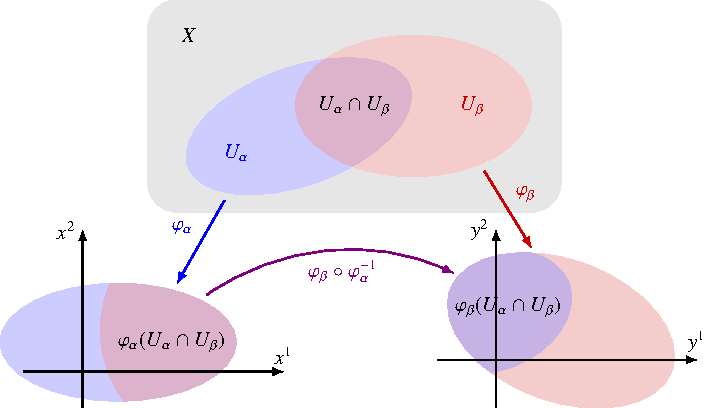
\includegraphics{chapters/020-koordinaten/images/koordinatenwechsel.pdf}
\caption{Koordinatenwechselabbildung $\varphi_\beta\circ\varphi_\alpha^{-1}$
zwischen zwei Karten $(U_\alpha,\varphi_\alpha)$ ({\color{blue}blau}) und
$(U_\beta,\varphi_\beta)$ ({\color{darkred}rot}).
\label{buch:koordinaten:diffmannig:fig:koordinatenwechsel}}
\end{figure}
%
Seien zwei Karten $(U_\alpha,\varphi_\alpha)$ und $(U_\beta,\varphi_\beta)$
gegeben derart, dass $U_\alpha\cap U_\beta$ nicht leer ist.
Auf der offenen Teilmenge $U_\alpha\cap U_\beta$ sind daher durch
die Abbildungen $\varphi_\alpha$ und $\varphi_\beta$ zwei
Koordinatensysteme gegegeben, die wir der Einfachheit halber wieder
mit den gleichen Symbolen bezeichnen\footnote{Genauer wäre, sie als
$\varphi_{\alpha|U_\alpha\cap U_\beta}$ und
$\varphi_{\beta|U_\alpha\cap U_\beta}$ zu bezeichnen, was jedoch
etwas schwerfällig ist.}.
Die Koordinatentransformation ist die Abbildung
\[
\varphi_\beta\circ\varphi_\alpha^{-1}
\colon
\varphi_\alpha(U_\alpha\cap U_\beta)
\to
\varphi_\beta(U_\alpha\cap U_\beta)
:
(x_\beta^1,\dots,x_\beta^n)
\mapsto
(x_\alpha^1,\dots,x_\alpha^n)
\]
(Abbildung~\ref{buch:koordinaten:diffmannig:fig:koordinatenwechsel}).
Sie heisst der {\em Kartenwechsel} von der Karte $(U_\beta,\varphi_\beta)$
zur Karte $(U_\beta,\varphi_\beta)$.
\index{Kartenwechsel}%

\begin{definition}[Atlas]
Ein {\em Atlas} ist eine Familie $(U_\alpha,\varphi_\alpha)_{\alpha\in I}$
von Karten derart, dass die Kartenwechwechsel
$\varphi_\alpha\circ\varphi_\beta^{-1}$ Homöomorphismen
für alle $\alpha,\beta\in I$ sind, für die
$U_\alpha\cap U_\beta\ne \emptyset$ ist.
\end{definition}

\begin{definition}[differenzierbarer Atlas]
Ein {\em differenzierbarer Atlas} ist ein Atlas, dessen
Kartenwechsel differenzierbar sind.
\end{definition}

Zu einer stetigen Struktur auf $X$ gehört der Atlas $(X,\varphi)$,
wobei $\varphi$ alle Koordinatensysteme der stetigen Struktur druchläuft.
Ist sogar eine differenzierbare Struktur auf der Menge $X$ gegeben,
wie sie in
Definition~\ref{buch:koordinaten:koordinaten:definition:diffbareestruktur}
definiert worden ist, dann bilden die Karten $(X,\varphi)$, wobei
$\varphi$ die Koordinatensysteme der differenzierbaren Struktur
durchläuft, einen differenzierbaren Atlas.

Für die Kugeloberfläche ist es nicht möglich, ein Koordinatensystem
zu finden, welches die ganze Kugeloberfläche abdeckt.
Dieses Phänomen trifft auch bei vielen anderen geometrischen Formen ein.
Ein Atlas ermöglicht, sich bei der Konstruktion auf lokale Betrachtungen
in der Umgegung eines Punktes zu beschränken.

\begin{definition}[differenzierbare Mannigfaltigkeit]
Eine {\em differenzierbare Mannigfaltigkeit} ist eine Menge $X$, die überdeckt
wird von den Definitionsgebieten eines differenzierbaren Atlas auf $X$.
\index{differenzierbare Mannigfaltigkeit}%
\index{Mannigfaltigkeit!differenzierbar}%
\end{definition}

Nach dieser Definition müsste die zweidimensionale Kugeloberfläche eine
differenzierbare Mannigfaltigkeit sein.
Das nachfolgende Beispiel zeigt, wie ein differenzierbarer Atlas
für die Kugeloberfläche gefunden werden kann.

\begin{beispiel}
Um zu zeigen, dass die zweidimensionale Kugeloberfläche
\[
S^2
=
\{
(x,y,z)\in\mathbb{R}^3
\mid
x^2 + y^2 + z^2 = 1
\}
\]
eine differenzierbare Mannigfaltigkeit ist, muss ein differenzierbare
Atlas konstruiert werden.
Dazu sind mindestens zwei Karten notwendig.
Wir konstruieren die Karten als stereographische Projektion von den
beiden Polen $N=(0,0,1)$ und $S=(0,0,-1)$ aus.
Als Definitionsbereich der Karten verwenden wir
\[
U_+
=
S^2\setminus \{ (0,0,1)\}
\qquad\text{und}\qquad
U_-
=
S^2\setminus \{ (0,0,-1)\}.
\]
Als Kartenabbildungen verwenden wir
\[
\varphi_+
\colon
(x,y,z)
\mapsto
\frac{1}{1-z}
(x,y)
\qquad\text{und}\qquad
\varphi_-
\colon
(x,y,z)
\mapsto
\frac{1}{1+z}
(x,y).
\]



Die Umkehrabbildungen sind etwas kompliziert auszudrücken, werden
aber auch nicht wirklich benötigt, nur die Zusammensetzung
$\varphi_{\mp}\circ\varphi_{\pm}^{-1}$ müssen berechnet daraufhin
untersucht werden, ob sie differenzierbar sind.
%
% fig-stereowechsel.tex
%
% (c) 2024 Prof Dr Andreas Müller
%
\begin{figure}
\centering
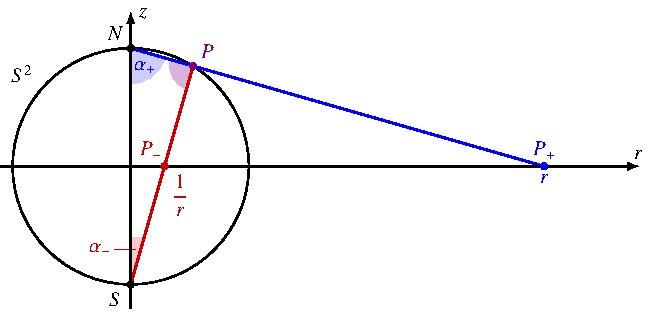
\includegraphics{chapters/020-koordinaten/images/stereowechsel.pdf}
\caption{Die stereographische Projektion $\varphi_+$ vom Nordpol
der Kugel aus bildet den Kugelpunkt $P$ auf den Punkt $P_+$ ab, die 
stereographische Projektion vom Südpol bildet ihn auf $P_-$ ab.
Die Kartenwechselabbildung $\varphi_-\circ\varphi_+^{-1}$ bildet $P_+$
auf $P_-$ ab.
Da $P$ auf dem Thales-Kreis über der Strecke $NS$ liegt, ist der Winkel
bei $P$ ein rechter Winkel und die Winkel $\alpha_+$ und $\alpha_-$
sind komplementär.
Es folgt, dass das Produkt der $r$-Koordinaten der Punkte $1$ ist.
\label{buch:koordinaten:diffmannig:fig:stereowechsel}}
\end{figure}
%
Die ist mit einem viel einfacheren geometrischen Argument möglich,
welches in Abbildung~\ref{buch:koordinaten:diffmannig:fig:stereowechsel}
erklärt wird.
Die Karte $\varphi_+$ bildet $P$ auf $P_+$ ab, $\varphi_-$ bildet
$P$ auf $P_-$ ab.
Da $P$ auf dem Thales-Kreis über der Strecke $NS$ liegt, ist der Winkel
$P$ ein rechter Winkel und die Winkel $\alpha_+$ und $\alpha_-$ sind
komplementär.
Die $r$-Koordinate von $P_-$ ist 
\[
\tan \alpha_-
=
\cot \alpha_+
=
\frac1{\tan\alpha_+}
=
\frac1{r}.
\]
Daraus lässt sich ableiten, dass die Kartenwechselabbildung
\[
\varphi_-\circ\varphi_+^{-1}
\colon
V_+\cap V_- \to V_-\cap V_+
:
(x^1_+,x^2_+)
\mapsto
\frac{1}{(x_+^1)^2 + (x_+^2)^2}(x_+^1,x_+^2)
\]
ist, die ganz offensichtlich differenzierbar ist, solange der 
Nenner nicht verschwindet.
\end{beispiel}

